% =====================================================================
%  IASTAM 6.0 -- Track 4, Problem 7 -- TECHNICAL PLAN & RELIABILITY REVIEW
%  Beamer + TikZ + pgfplots. Compile with pdflatex or on Overleaf.
%
%  Conventions used in this deck:
%   * [SIM]  = output of our simulator with a SYNTHETIC workload (not real data)
%   * [LIT]  = number taken from the cited paper/source
%   * TARGET = a goal we set, not a result
% =====================================================================
\documentclass[aspectratio=169,10pt]{beamer}

\usetheme{Madrid}
\usecolortheme{default}
\setbeamertemplate{navigation symbols}{}

\usepackage[utf8]{inputenc}
\usepackage[T1]{fontenc}
\usepackage{lmodern}
\usepackage{booktabs}
\usepackage{tabularx}
\usepackage{array}
\usepackage{amsmath,amssymb}
\usepackage{tikz}
\usepackage{pgfplots}
\pgfplotsset{compat=1.18}
\usetikzlibrary{positioning,arrows.meta,shapes.geometric,calc,fit,backgrounds}

% ---------- Colours ----------
\definecolor{space}{HTML}{0B2545}
\definecolor{ocean}{HTML}{1B6CA8}
\definecolor{sky}{HTML}{8DB8E0}
\definecolor{accent}{HTML}{E07A1F}
\definecolor{good}{HTML}{2E8B57}
\definecolor{bad}{HTML}{C0392B}
\definecolor{muted}{HTML}{6B7280}
\definecolor{paper}{HTML}{F3F6FA}

\setbeamercolor{structure}{fg=ocean}
\setbeamercolor{palette primary}{bg=space,fg=white}
\setbeamercolor{palette secondary}{bg=ocean,fg=white}
\setbeamercolor{palette tertiary}{bg=space,fg=white}
\setbeamercolor{frametitle}{bg=space,fg=white}
\setbeamercolor{title}{bg=space,fg=white}
\setbeamercolor{block title}{bg=ocean,fg=white}
\setbeamercolor{block body}{bg=paper,fg=black}
\setbeamercolor{block title alerted}{bg=accent,fg=white}
\setbeamercolor{block body alerted}{bg=accent!8,fg=black}
\setbeamercolor{block title example}{bg=good,fg=white}
\setbeamercolor{block body example}{bg=good!8,fg=black}

\newcolumntype{L}{>{\raggedright\arraybackslash}X}
\newcolumntype{P}[1]{>{\raggedright\arraybackslash}p{#1}}

\newcommand{\phisat}[1]{$\Phi$-sat-#1}
\newcommand{\src}[1]{{\scriptsize\color{muted}[#1]}}
\newcommand{\hl}[1]{\textbf{\color{accent}#1}}
\newcommand{\ok}{\textcolor{good}{$\checkmark$}}
\newcommand{\warn}{\textcolor{accent}{\textbf{!}}}
\newcommand{\SIMtag}{\textcolor{ocean}{\textbf{[SIM]}}}
\newcommand{\LITtag}{\textcolor{muted}{\textbf{[LIT]}}}

\title[Problem 7 -- Technical Plan]{Technical Plan \& Reliability Review}
\subtitle{IASTAM 6.0 -- Track 4, Problem 7: Transmitting Information, Not Raw Data}
\author[Team]{Team \textit{<Your Team Name>}}
\institute[IASTAM 6.0]{Computer Engineering -- 2nd year}
\date{18 September 2026}

\begin{document}

% =====================================================================
\begin{frame}
  \titlepage
\end{frame}

\begin{frame}{Outline}
  \tableofcontents
  \vspace{3mm}
  {\footnotesize\color{muted}
  Legend used in every slide: \SIMtag{} = our simulator with a synthetic workload \quad
  \LITtag{} = number from a cited source \quad \textbf{TARGET} = a goal, not a result.}
\end{frame}

% =====================================================================
\section{Where We Are}
% =====================================================================

\begin{frame}{System architecture and data contracts}
\centering
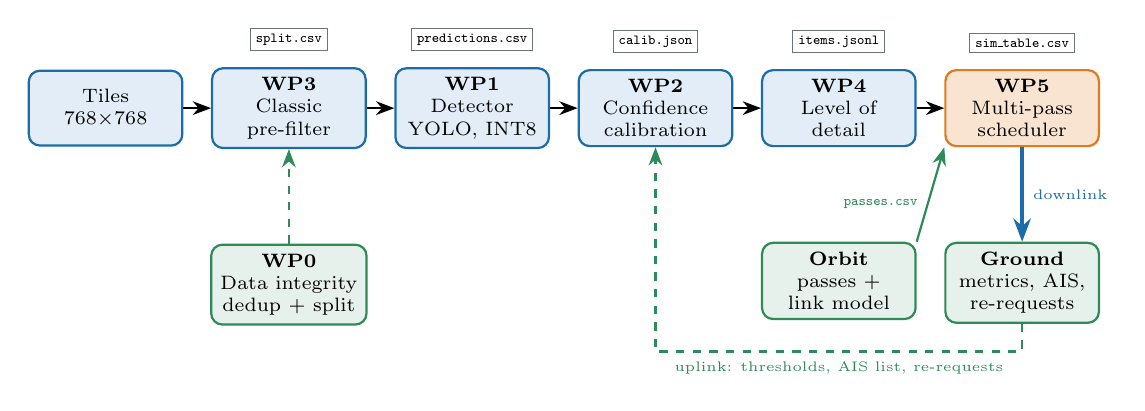
\begin{tikzpicture}[
  st/.style={draw=ocean,thick,rounded corners,fill=sky!25,minimum width=1.95cm,minimum height=0.95cm,align=center,font=\scriptsize},
  gd/.style={draw=good,thick,rounded corners,fill=good!12,minimum width=1.95cm,minimum height=0.95cm,align=center,font=\scriptsize},
  file/.style={draw=muted,fill=white,font=\tiny\ttfamily,inner sep=2pt},
  arr/.style={-{Stealth},thick},
  node distance=3.5mm]
  \node[st] (t)  {Tiles\\768$\times$768};
  \node[st,right=of t]  (p)  {\textbf{WP3}\\Classic\\pre-filter};
  \node[st,right=of p]  (d)  {\textbf{WP1}\\Detector\\YOLO, INT8};
  \node[st,right=of d]  (c)  {\textbf{WP2}\\Confidence\\calibration};
  \node[st,right=of c]  (l)  {\textbf{WP4}\\Level of\\detail};
  \node[st,right=of l,fill=accent!20,draw=accent] (s)  {\textbf{WP5}\\Multi-pass\\scheduler};
  \node[gd,below=12mm of s] (g)  {\textbf{Ground}\\metrics, AIS,\\re-requests};
  \node[gd,below=12mm of l] (o)  {\textbf{Orbit}\\passes +\\link model};
  \node[gd,below=12mm of p] (a)  {\textbf{WP0}\\Data integrity\\dedup + split};
  \draw[arr] (t) -- (p);
  \draw[arr] (p) -- (d);
  \draw[arr] (d) -- (c);
  \draw[arr] (c) -- (l);
  \draw[arr] (l) -- (s);
  \draw[arr,ocean,very thick] (s) -- node[right,font=\tiny]{downlink} (g);
  \draw[arr,good] (o.north east) -- node[left,font=\tiny,pos=0.4]{\texttt{passes.csv}} (s.south west);
  \draw[arr,good,dashed] (a.north) -- (p.south);
  \draw[arr,good,dashed] (g.south) -- ++(0,-0.35) -| node[pos=0.25,below,font=\tiny]{uplink: thresholds, AIS list, re-requests} (c.south);
  \node[file,above=2mm of p] {split.csv};
  \node[file,above=2mm of d] {predictions.csv};
  \node[file,above=2mm of c] {calib.json};
  \node[file,above=2mm of l] {items.jsonl};
  \node[file,above=2mm of s] {sim\_table.csv};
\end{tikzpicture}
\vspace{3mm}

{\footnotesize Each box is a work package (WP) with one owner and \textbf{one file as its interface}, so the team can work in parallel.}
\end{frame}

% ---------------------------------------------------------------------
\begin{frame}{Already built and tested (repository \texttt{code/})}
\footnotesize
\renewcommand{\arraystretch}{1.15}
\begin{tabularx}{\textwidth}{@{}P{3.1cm} L P{3.4cm}@{}}
\toprule
\textbf{Module} & \textbf{What it does} & \textbf{Status} \\
\midrule
\texttt{sat7/rle.py} & Airbus RLE masks $\leftrightarrow$ boxes $\leftrightarrow$ YOLO labels, IoU & \ok{} unit-tested \\
\texttt{sat7/prefilter.py} & HSV cloud mask (+ opening), top-hat + Otsu, opening, connected components, watershed, Canny & \ok{} tested on synthetic tiles \\
\texttt{sat7/orbit.py} & SGP4/Skyfield passes over Sfax, $C_{\text{pass}}=\sum_k R_k\Delta t_k$ & \ok{} tested \\
\texttt{sat7/scheduler.py} & Encoders (raw, fixed patch, LoD) + policies (no-buffer, FIFO, value-greedy) & \ok{} tested \\
\texttt{scripts/airbus\_to\_yolo.py} & Airbus $\rightarrow$ YOLO dataset + \texttt{data.yaml} & \ok{} end-to-end on a mock folder \\
\texttt{scripts/simulate\_day.py} & 5 strategies, load sweep, Wilson 95\% CIs & \ok{} runs in $\sim$40\,s \\
\bottomrule
\end{tabularx}
\vspace{2mm}
\begin{exampleblock}{Test suite}
\footnotesize 17 automated tests pass (including a regression test for a bug the tests caught: partly cloudy tiles were dropped with visible ships inside).
\end{exampleblock}
\end{frame}

% ---------------------------------------------------------------------
\begin{frame}{Real orbit geometry: contact windows over Sfax}
\begin{columns}[c]
\column{0.6\textwidth}
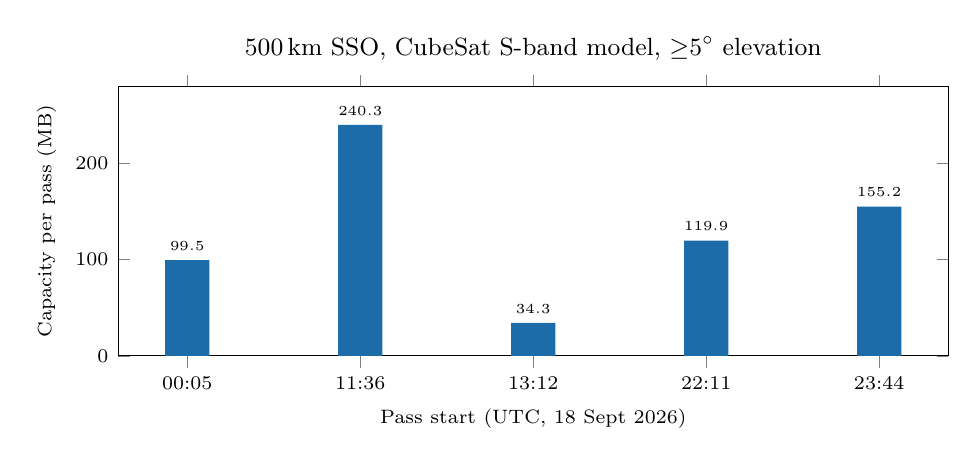
\begin{tikzpicture}
\begin{axis}[
  ybar, bar shift=0pt, width=\linewidth, height=5cm,
  ymin=0, ymax=280,
  ylabel={Capacity per pass (MB)}, ylabel style={font=\scriptsize},
  symbolic x coords={P1,P2,P3,P4,P5},
  xtick=data, xticklabels={00:05,11:36,13:12,22:11,23:44},
  xlabel={Pass start (UTC, 18 Sept 2026)}, xlabel style={font=\scriptsize},
  ticklabel style={font=\scriptsize},
  nodes near coords, nodes near coords style={font=\tiny},
  bar width=16pt,
  title={\small 500\,km SSO, CubeSat S-band model, $\geq$5$^\circ$ elevation},
]
\addplot[fill=ocean,draw=none] coordinates {(P1,99.5) (P2,240.3) (P3,34.3) (P4,119.9) (P5,155.2)};
\end{axis}
\end{tikzpicture}
\column{0.38\textwidth}
\footnotesize
\begin{itemize}
  \item \textbf{5 passes / day}, 34.2 min of contact in total
  \item \hl{Longest gap without contact: 11.4 h}
  \item Capacity varies $7\times$ between passes (elevation)
  \item Link cap 8\,Mbps is consistent with CubeSat S-band transmitters (4.3--10\,Mbps) \LITtag
\end{itemize}
\vspace{1mm}
\begin{alertblock}{Consequence}
\footnotesize Buffering across passes is not optional, and a pass can carry very different amounts of data.
\end{alertblock}
\end{columns}
\end{frame}

% ---------------------------------------------------------------------
\begin{frame}{First results \SIMtag: one day, congested downlink}
\begin{columns}[T]
\column{0.5\textwidth}
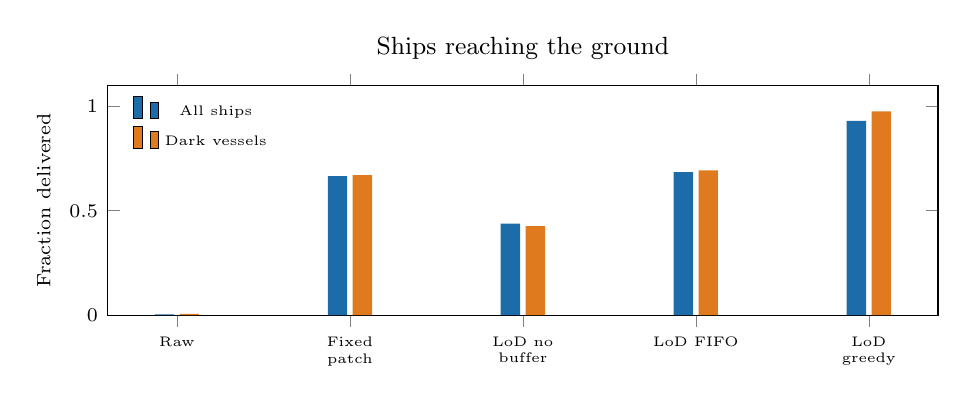
\begin{tikzpicture}
\begin{axis}[
  ybar, width=\linewidth, height=4.5cm,
  ymin=0, ymax=1.1,
  ylabel={Fraction delivered}, ylabel style={font=\scriptsize},
  symbolic x coords={S1,S2,S3,S4,S5},
  xtick=data,
  xticklabels={Raw,Fixed patch,LoD no buffer,LoD FIFO,LoD greedy},
  xticklabel style={font=\tiny,text width=1.1cm,align=center},
  yticklabel style={font=\scriptsize},
  bar width=7pt,
  legend style={font=\tiny,at={(0.02,0.98)},anchor=north west,draw=none,fill=none},
  title={\small Ships reaching the ground},
]
\addplot[fill=ocean,draw=none] coordinates {(S1,0.004) (S2,0.666) (S3,0.439) (S4,0.685) (S5,0.930)};
\addplot[fill=accent,draw=none] coordinates {(S1,0.006) (S2,0.671) (S3,0.426) (S4,0.693) (S5,0.976)};
\legend{All ships, Dark vessels}
\end{axis}
\end{tikzpicture}
\column{0.5\textwidth}
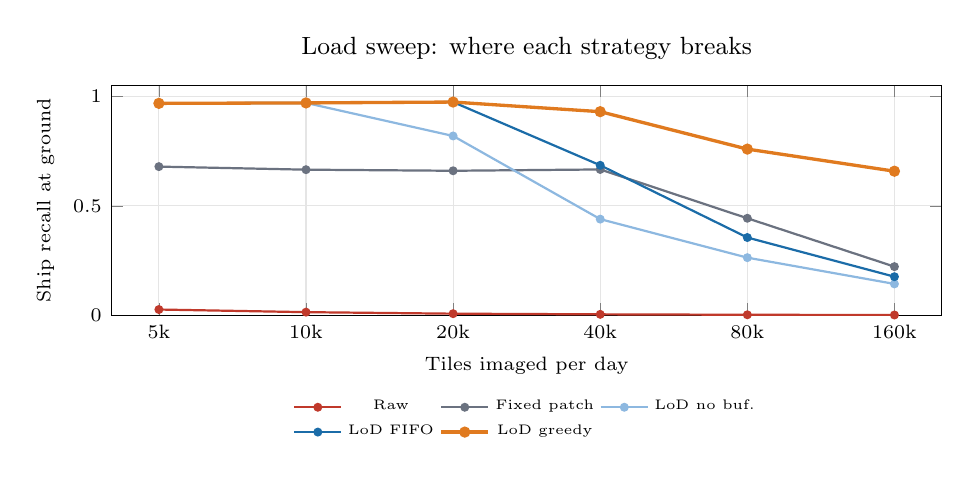
\begin{tikzpicture}
\begin{axis}[
  width=\linewidth, height=4.5cm,
  xmode=log, xmin=4000, xmax=200000, ymin=0, ymax=1.05,
  xtick={5000,10000,20000,40000,80000,160000},
  xticklabels={5k,10k,20k,40k,80k,160k},
  xlabel={Tiles imaged per day}, xlabel style={font=\scriptsize},
  ylabel={Ship recall at ground}, ylabel style={font=\scriptsize},
  ticklabel style={font=\scriptsize},
  grid=major, grid style={gray!20},
  legend style={font=\tiny,at={(0.5,-0.32)},anchor=north,legend columns=3,draw=none},
  title={\small Load sweep: where each strategy breaks},
]
\addplot[bad,thick,mark=*,mark size=1.2pt] coordinates {(5000,0.026) (10000,0.014) (20000,0.007) (40000,0.004) (80000,0.002) (160000,0.001)};
\addplot[muted,thick,mark=*,mark size=1.2pt] coordinates {(5000,0.679) (10000,0.665) (20000,0.660) (40000,0.666) (80000,0.443) (160000,0.222)};
\addplot[sky,thick,mark=*,mark size=1.2pt] coordinates {(5000,0.968) (10000,0.970) (20000,0.819) (40000,0.439) (80000,0.263) (160000,0.143)};
\addplot[ocean,thick,mark=*,mark size=1.2pt] coordinates {(5000,0.968) (10000,0.970) (20000,0.974) (40000,0.685) (80000,0.355) (160000,0.176)};
\addplot[accent,very thick,mark=*,mark size=1.4pt] coordinates {(5000,0.968) (10000,0.970) (20000,0.974) (40000,0.930) (80000,0.759) (160000,0.658)};
\legend{Raw,Fixed patch,LoD no buf.,LoD FIFO,LoD greedy}
\end{axis}
\end{tikzpicture}
\end{columns}
\vspace{-1mm}
{\scriptsize LoD FIFO vs LoD greedy send the \emph{same} data: 68.5\% $\rightarrow$ 93.0\% at 40k tiles/day is the effect of the scheduler alone.
\textcolor{bad}{Synthetic workload: these are not real-data results.}}
\end{frame}

% =====================================================================
\section{Reliability Review}
% =====================================================================

\begin{frame}{Checking our choices against evidence}
\scriptsize
\renewcommand{\arraystretch}{1.12}
\begin{tabularx}{\textwidth}{@{}P{2.7cm} L c P{3.3cm}@{}}
\toprule
\textbf{Choice} & \textbf{Evidence \LITtag} & & \textbf{Consequence for us} \\
\midrule
Airbus dataset & SPOT imagery, 1.5\,m; 768$\times$768 crops; 22.1\% contain ships; box diagonals 1--380\,px (median 43\,px) & \ok & Good fit; plan for tiny \emph{and} huge ships \\
Airbus crops & Neighbouring crops overlap: the same ship appears in several images & \warn & Leakage risk $\rightarrow$ WP0 \\
YOLOv8 on Airbus & 88\% mAP reported (metric definition not detailed) & \ok & Realistic target \\
INT8 quantization & 1.5--3.3$\times$ faster, 3--7\% mAP50-95 drop (TensorRT, YOLO n--x) & \warn & Measure per ship size $\rightarrow$ WP1 \\
Detector confidence & Detectors are intrinsically miscalibrated; temperature scaling cut ECE 6.78\%$\rightarrow$2.31\% (YOLO-World) & \warn & Our LoD thresholds need calibration $\rightarrow$ WP2 \\
Link model & CubeSat S-band 4.3--10\,Mbps; X-band 100--400\,Mbps & \ok & Our 8\,Mbps cap is realistic \\
AIS as reference & Gaps from reception congestion; spoofed tracks exist & \warn & ``No AIS match'' = priority, not accusation \\
Greedy scheduling & Optimal for fractional knapsack; not for 0/1 items & \warn & Measure the optimality gap $\rightarrow$ WP5 \\
\bottomrule
\end{tabularx}
\vspace{1mm}
{\tiny\color{muted} Sources: Faudi (Airbus); arXiv 2406.11319; Relova (Airbus EDA); arXiv 2503.14534; arXiv 2508.19600; K\"uppers et al.\ 2022; Appl.\ Sci.\ 15(22) 2025; ISISPACE / AAC Clyde / satsearch; Global Fishing Watch; Kellerer et al.\ 2004.}
\end{frame}

% ---------------------------------------------------------------------
\begin{frame}{Five weaknesses found in our own work -- and the fix}
\footnotesize
\renewcommand{\arraystretch}{1.2}
\begin{tabularx}{\textwidth}{@{}c P{4.1cm} L c@{}}
\toprule
& \textbf{Weakness} & \textbf{Fix} & \textbf{WP} \\
\midrule
1 & All scheduler results use a \textbf{synthetic workload} & Feed real detections from Airbus test images (matched to ground truth) & 1, 5 \\
2 & \textbf{Fixed-patch baseline is unfair}: in our simulation it ignores coastal ships by construction & Give every baseline the same coastal handling; compare only the level-of-detail choice & 5 \\
3 & LoD thresholds (0.4 / 0.9) assume \textbf{calibrated confidences} & Calibrate on the validation split; report reliability diagram + ECE & 2 \\
4 & Top-hat kernel (31\,px) \textbf{smaller than big ships} (up to 380\,px diagonal) $\Rightarrow$ large ships get cut & Size the structuring element from the Airbus beam distribution, or use two scales & 3 \\
5 & Crop overlap $\Rightarrow$ \textbf{inflated test scores} & Perceptual-hash duplicate groups; split by group & 0 \\
\bottomrule
\end{tabularx}
\vspace{2mm}
\begin{alertblock}{Why this slide matters}
\footnotesize Finding and fixing our own weaknesses before the jury does is the strongest evidence of ``understanding'' and ``methodology''.
\end{alertblock}
\end{frame}

% =====================================================================
\section{Technical Plan}
% =====================================================================

\begin{frame}{Work packages}
\scriptsize
\renewcommand{\arraystretch}{1.18}
\begin{tabularx}{\textwidth}{@{}l P{2.9cm} L P{3.6cm}@{}}
\toprule
\textbf{WP} & \textbf{Name} & \textbf{Output (interface file)} & \textbf{Acceptance (TARGET)} \\
\midrule
0 & Data integrity & \texttt{split.csv} with duplicate groups & 0 near-duplicate pairs across splits \\
1 & Detector & \texttt{predictions.csv}; ONNX FP32 / INT8; latency & Recall $\geq$ 0.85 @ IoU 0.5; INT8 drop $\leq$ 3 pts mAP50 \\
2 & Calibration & \texttt{calib.json} (temperature or isotonic) & ECE reduced; thresholds on calibrated $\hat p$ \\
3 & Classic pre-filter & Tuned config + real-data report & $\geq$ 99\% of ships on kept tiles \\
4 & LoD encoder & \texttt{items.jsonl} with \emph{measured} sizes and values & Sizes/values measured, not assumed \\
5 & Scheduler & \texttt{sim\_table.csv}, gap study, sensitivity & Gap to exact optimum reported \\
6 & Reliability & FMEA, fault-injection tests, audit sampling & All failure modes have a tested fallback \\
7 & Integration \& demo & End-to-end script + dashboard & One command from tiles to charts \\
\bottomrule
\end{tabularx}
\end{frame}

% ---------------------------------------------------------------------
\begin{frame}{WP0 -- Data integrity \quad \& \quad WP1 -- Detector}
\begin{columns}[T]
\column{0.47\textwidth}
\begin{block}{WP0: no leakage}
\footnotesize
\begin{enumerate}
  \item Perceptual hash (pHash) of every image and of its 4 half-tiles
  \item Hamming distance $\leq$ threshold $\Rightarrow$ same group (union--find)
  \item Split \textbf{by group}: train / val / test = 80 / 10 / 10
  \item Keep negatives: 0.25 empty tile per ship tile
\end{enumerate}
\src{method: perceptual hashing, arXiv 2304.02296 -- found 93\% val/train leakage in another geospatial dataset}
\end{block}
\column{0.51\textwidth}
\begin{block}{WP1: detector}
\footnotesize
\begin{itemize}
  \item YOLOv8n (or YOLO11n), \texttt{imgsz}=768, Kaggle / Colab GPU
  \item Metrics by ship size: small ($<$32\,px), medium, large
  \item Export ONNX \textbf{FP32 vs INT8}, same test split
  \item CPU latency (median, P90) on the laptop, labelled as such
  \item Save \emph{all} boxes with score $\geq$ 0.05 (needed for calibration)
\end{itemize}
\end{block}
\end{columns}
\vspace{2mm}
\begin{exampleblock}{Why tiles, not full frames}
\footnotesize Airbus images are already 768$\times$768 tiles, so no slicing is needed. For full satellite frames, tiled inference (SAHI) raised AP by 5--7 points on aerial datasets \LITtag.
\end{exampleblock}
\end{frame}

% ---------------------------------------------------------------------
\begin{frame}{WP2 -- Confidence calibration (the LoD rule depends on it)}
\begin{columns}[c]
\column{0.5\textwidth}
\footnotesize
\textbf{Problem.} Our rule ``confidence $>$ 0.9 $\Rightarrow$ metadata only'' is meaningful only if 0.9 really means ``90\% of such boxes are ships''.\\[2mm]
\textbf{Method.}
\begin{enumerate}
  \item Match val predictions to ground truth (IoU $\geq$ 0.5) $\Rightarrow$ label 1/0
  \item Fit temperature $T$ (or isotonic regression) on these labels
  \item Report \textbf{reliability diagram} + ECE before/after
  \item Choose LoD thresholds on calibrated $\hat p$
\end{enumerate}
\[ \text{ECE} = \sum_{b} \tfrac{|B_b|}{N}\,\big|\,\text{acc}(B_b)-\text{conf}(B_b)\big| \]
\column{0.48\textwidth}
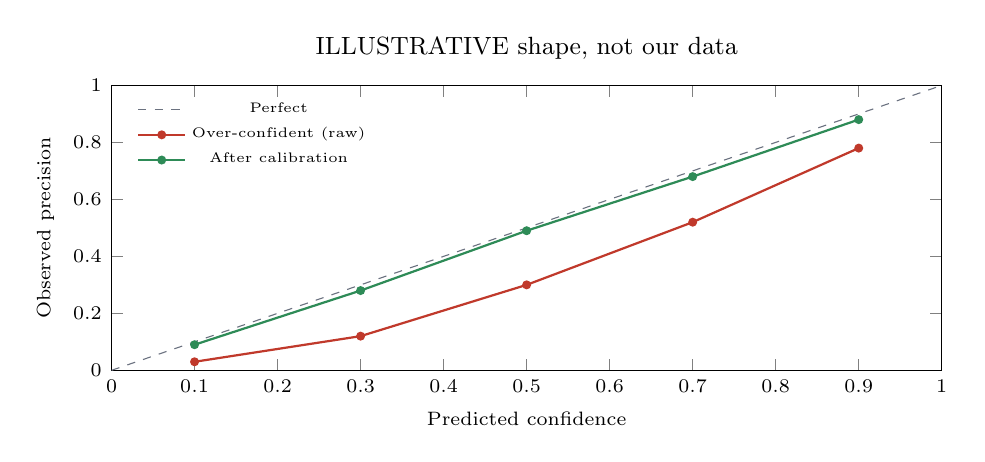
\begin{tikzpicture}
\begin{axis}[
  width=\linewidth, height=5.2cm, xmin=0, xmax=1, ymin=0, ymax=1,
  xlabel={Predicted confidence}, ylabel={Observed precision},
  xlabel style={font=\scriptsize}, ylabel style={font=\scriptsize},
  ticklabel style={font=\scriptsize},
  legend style={font=\tiny,at={(0.02,0.98)},anchor=north west,draw=none,fill=none},
  title={\small ILLUSTRATIVE shape, not our data},
]
\addplot[muted,dashed,domain=0:1] {x};
\addplot[bad,thick,mark=*,mark size=1.2pt] coordinates {(0.1,0.03) (0.3,0.12) (0.5,0.30) (0.7,0.52) (0.9,0.78)};
\addplot[good,thick,mark=*,mark size=1.2pt] coordinates {(0.1,0.09) (0.3,0.28) (0.5,0.49) (0.7,0.68) (0.9,0.88)};
\legend{Perfect, Over-confident (raw), After calibration}
\end{axis}
\end{tikzpicture}
\end{columns}
\end{frame}

% ---------------------------------------------------------------------
\begin{frame}{WP3 -- Classic pre-filter on real Airbus tiles}
\begin{columns}[T]
\column{0.5\textwidth}
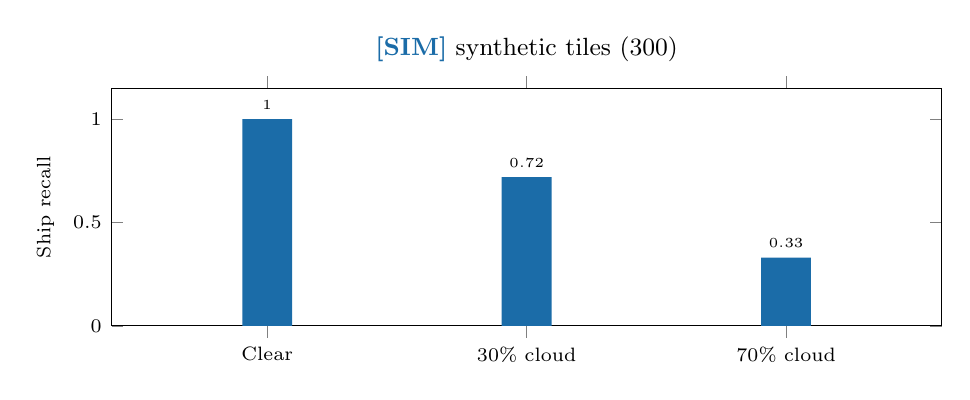
\begin{tikzpicture}
\begin{axis}[
  ybar, bar shift=0pt, width=\linewidth, height=4.6cm,
  ymin=0, ymax=1.15,
  ylabel={Ship recall}, ylabel style={font=\scriptsize},
  symbolic x coords={C0,C30,C70},
  xtick=data, xticklabels={Clear,30\% cloud,70\% cloud},
  ticklabel style={font=\scriptsize},
  nodes near coords, nodes near coords style={font=\tiny},
  bar width=18pt, enlarge x limits=0.3,
  title={\small \SIMtag{} synthetic tiles (300)},
]
\addplot[fill=ocean,draw=none] coordinates {(C0,1.00) (C30,0.72) (C70,0.33)};
\end{axis}
\end{tikzpicture}
{\scriptsize Clear sky: 191/191 ships found. In cloudy tiles many ships are painted \emph{under} the cloud.}
\column{0.48\textwidth}
\begin{block}{Plan on real data}
\footnotesize
\begin{itemize}
  \item Structuring element sized from data: top-hat SE $>$ widest ship beam (weakness 4)
  \item Tune thresholds on \textbf{val}, report on \textbf{test}
  \item Safety metric: share of ships on \emph{kept} tiles -- TARGET $\geq$ 99\%
  \item Saving metric: share of empty tiles dropped
  \item Log failure cases: waves, sun glint, wakes, cloud edges
\end{itemize}
\end{block}
\end{columns}
\vspace{1mm}
\begin{alertblock}{Role in the system}
\footnotesize The pre-filter only saves compute. It must never be the last line of defence: kept tiles still go to the detector, dropped tiles still leave a thumbnail.
\end{alertblock}
\end{frame}

% ---------------------------------------------------------------------
\begin{frame}{WP4 -- Level of detail with \emph{measured} value, not assumed}
\begin{columns}[T]
\column{0.52\textwidth}
\begin{block}{Idea}
\footnotesize The value of sending a ship at level $\ell$ is the probability that the ground can still confirm it:
\[ g(\ell) = P\big(\text{detected on the decoded payload} \mid \text{level } \ell\big) \]
Measured by \textbf{re-running the detector} on each compressed chip / ROI.
\end{block}
\begin{block}{Procedure}
\footnotesize
\begin{enumerate}
  \item For each test ship: crop chips at 3 sizes
  \item Encode JPEG / JPEG2000 at several qualities
  \item Record \textbf{real bytes} and detection success
  \item Fit $g(\ell)$ and bytes$(\ell)$ tables
\end{enumerate}
\end{block}
\column{0.46\textwidth}
\footnotesize
\renewcommand{\arraystretch}{1.25}
\begin{tabularx}{\linewidth}{@{}l L@{}}
\toprule
\textbf{Level} & \textbf{Content} \\
\midrule
L0 & lat, lon, length, heading, $\hat p$ ($\sim$40\,B) \\
L1 & small chip, low quality \\
L2 & progressive ROI (can be truncated) \\
Tile & coastal / port tile, progressive \\
Thumb & low-resolution tile (safety net) \\
\bottomrule
\end{tabularx}
\vspace{2mm}
\begin{exampleblock}{Why it matters}
\footnotesize Replaces our assumed sizes and values with numbers the jury can check.
\end{exampleblock}
\end{columns}
\end{frame}

% ---------------------------------------------------------------------
\begin{frame}{WP5 -- Scheduler as an optimisation problem}
\begin{columns}[T]
\column{0.53\textwidth}
\begin{block}{Formulation (one pass)}
\footnotesize
\[ \max_{x_i\in[0,1]} \sum_i v_i\, h_i(x_i) \quad \text{s.t.} \quad \sum_i b_i\, x_i \leq C_{\text{pass}} \]
$x_i$: fraction of item $i$ sent ($x_i\in\{0,1\}$ unless progressive), $h_i$ concave (e.g.\ $\sqrt{x}$), $b_i$ bytes, $v_i$ value with aging.
\end{block}
\begin{block}{Theory we rely on}
\footnotesize
\begin{itemize}
  \item Fractional + linear value: greedy by $v/b$ is \textbf{optimal}
  \item Concave $h_i$: greedy on marginal value per byte (water-filling) is optimal in the continuous case
  \item 0/1 items: greedy alone can be poor; greedy + best single item $\geq \tfrac12$ OPT
\end{itemize}
\src{Kellerer, Pferschy, Pisinger, \emph{Knapsack Problems}, 2004}
\end{block}
\column{0.45\textwidth}
\begin{block}{Experiments}
\footnotesize
\begin{enumerate}
  \item \textbf{Exact DP} on small passes $\Rightarrow$ optimality gap of greedy
  \item \textbf{Offline LP upper bound} over the whole day (knows the future) $\Rightarrow$ cost of being online
  \item Fair baselines (weakness 2)
  \item Sensitivity: link share, dark weight, aging $\alpha$, storage
  \item 5 random seeds, Wilson 95\% CI, median/P90 latency
\end{enumerate}
\end{block}
\end{columns}
\end{frame}

% ---------------------------------------------------------------------
\begin{frame}{WP6 -- Failure modes and effects (FMEA)}
\scriptsize
\renewcommand{\arraystretch}{1.12}
\begin{tabularx}{\textwidth}{@{}P{2.9cm} P{2.9cm} P{2.5cm} L@{}}
\toprule
\textbf{Failure mode} & \textbf{Effect} & \textbf{How we detect it} & \textbf{Mitigation (tested)} \\
\midrule
Detector misses a ship & Ship never reported & Test recall; audit sampling & Thumbnail + raw ring buffer, ground re-request \\
Miscalibrated confidence & Wrong level of detail & ECE, reliability diagram & Calibration (WP2), recalibrate from ground \\
Domain shift (new sensor, sea state) & Silent recall drop & Audit sampling in orbit & Uplink new thresholds / model \\
INT8 degradation on small ships & Small ships lost & FP32 vs INT8 per size bucket & Keep FP16 for the small-ship head \\
AIS gap or spoofing & False ``dark'' flags / missed dark & Ground cross-check & ``Dark'' = priority only, human confirms \\
Pass capacity lower than predicted & Plan overflows & Link telemetry & Progressive items, re-plan each pass \\
Storage full & Data loss & Queue monitor & Drop lowest value-per-byte first \\
Software crash / bit flip & Pipeline stops & Watchdog & \textbf{Safe mode}: thumbnails + FIFO \\
Evaluation leakage & Over-optimistic paper & WP0 duplicate check & Group split \\
\bottomrule
\end{tabularx}
\end{frame}

% ---------------------------------------------------------------------
\begin{frame}{Reliability mechanisms we will implement and test}
\begin{columns}[T]
\column{0.33\textwidth}
\begin{block}{Audit sampling}
\footnotesize Downlink a random 1\% of raw tiles regardless of the AI decision.\\[1mm]
$\Rightarrow$ The ground gets an \textbf{unbiased estimate of in-orbit recall}, so a silent failure (domain shift) becomes visible.
\end{block}
\column{0.32\textwidth}
\begin{block}{Safe mode}
\footnotesize If the detector crashes, times out, or the watchdog fires:\\[1mm]
thumbnails + FIFO of the ring buffer.\\[1mm]
$\Rightarrow$ The mission degrades, it does not stop.
\end{block}
\column{0.33\textwidth}
\begin{block}{Fault injection}
\footnotesize Automated tests that:
\begin{itemize}
  \item drop a pass
  \item halve a pass capacity
  \item switch the detector off
  \item fill the storage
\end{itemize}
and check the fallback behaviour.
\end{block}
\end{columns}
\vspace{3mm}
\begin{alertblock}{Evidence that COTS computing is viable in LEO}
\footnotesize Raspberry Pi 4 and Atlas 200 flew 6 months on BUPT-1 with no radiation errors observed; computing used 30--40\% of the energy and long high-power tasks hit thermal limits \LITtag{} $\Rightarrow$ duty-cycled processing + safe mode.
\end{alertblock}
\end{frame}

% ---------------------------------------------------------------------
\begin{frame}{Evaluation protocol (mapped to the official criteria)}
\footnotesize
\renewcommand{\arraystretch}{1.2}
\begin{tabularx}{\textwidth}{@{}P{3.4cm} L P{3.6cm}@{}}
\toprule
\textbf{Official criterion} & \textbf{Our metric} & \textbf{Measured on} \\
\midrule
Data reduction rate & raw bytes / sent bytes & Airbus test + simulator \\
Preservation of useful information & Ship recall \emph{at the ground}; dark-vessel recall; value delivered & Real detections + simulator \\
Accuracy of results & Detector precision / recall / mAP50 by size; position error; ECE & Airbus test split \\
Latency & Capture $\rightarrow$ ground: median and P90 & Simulator with real passes \\
\bottomrule
\end{tabularx}
\vspace{2mm}
\begin{columns}[T]
\column{0.5\textwidth}
\begin{block}{Baselines}
\footnotesize Raw bent pipe $\cdot$ JPEG2000 all $\cdot$ cloud/empty filter ($\Phi$-sat-1 style) $\cdot$ fixed patch ($\Phi$-sat-2 style, \emph{fair version})
\end{block}
\column{0.48\textwidth}
\begin{block}{Statistics}
\footnotesize 5 seeds $\cdot$ Wilson 95\% CI for recalls $\cdot$ median / P90 latency $\cdot$ every assumption listed
\end{block}
\end{columns}
\end{frame}

% ---------------------------------------------------------------------
\begin{frame}{Timeline}
\centering
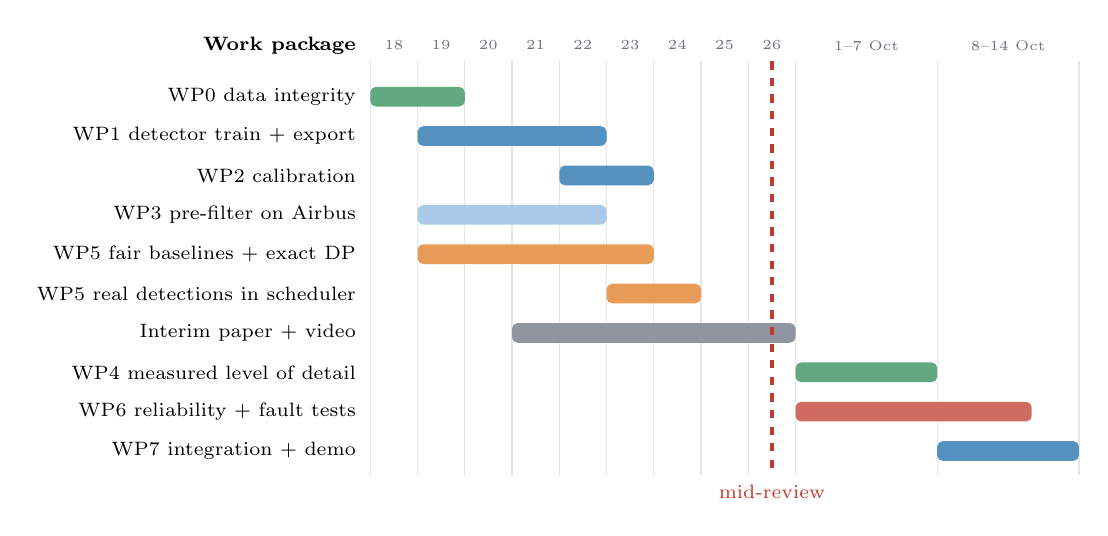
\begin{tikzpicture}[x=0.6cm,y=0.5cm]
  % day axis: 18 Sep ... 30 Sep then Oct weeks
  \foreach \dday [count=\dpos from 0] in {18,19,20,21,22,23,24,25,26} {
    \node[font=\tiny,muted] at (\dpos+0.5,0.6) {\dday};
    \draw[gray!20] (\dpos,0.2) -- (\dpos,-10.3);
  }
  \node[font=\tiny,muted] at (10.5,0.6) {1--7 Oct};
  \node[font=\tiny,muted] at (13.5,0.6) {8--14 Oct};
  \draw[gray!20] (9,0.2) -- (9,-10.3);
  \draw[gray!20] (12,0.2) -- (12,-10.3);
  \draw[gray!20] (15,0.2) -- (15,-10.3);
  \node[font=\scriptsize,anchor=east] at (-0.1,0.6) {\textbf{Work package}};
  \foreach \tname/\tstart/\tlen/\tcol [count=\trow] in {
      WP0 data integrity/0/2/good,
      WP1 detector train + export/1/4/ocean,
      WP2 calibration/4/2/ocean,
      WP3 pre-filter on Airbus/1/4/sky,
      WP5 fair baselines + exact DP/1/5/accent,
      WP5 real detections in scheduler/5/2/accent,
      Interim paper + video/3/6/muted,
      WP4 measured level of detail/9/3/good,
      WP6 reliability + fault tests/9/5/bad,
      WP7 integration + demo/12/3/ocean} {
    \node[font=\scriptsize,anchor=east] at (-0.1,-\trow+0.3) {\tname};
    \fill[\tcol!75,rounded corners=2pt] (\tstart,-\trow+0.05) rectangle (\tstart+\tlen,-\trow+0.55);
  }
  \draw[bad,very thick,dashed] (8.5,0.2) -- (8.5,-10.3) node[below,font=\scriptsize,bad] {mid-review};
\end{tikzpicture}
\end{frame}

% ---------------------------------------------------------------------
\begin{frame}{Definition of done for the mid-review (26 Sept)}
\begin{columns}[T]
\column{0.5\textwidth}
\begin{block}{Must have}
\footnotesize
\begin{itemize}
  \item[\ok] Leakage-free split (WP0)
  \item[\ok] Detector metrics on the test split, FP32 and INT8 (WP1)
  \item[\ok] Pre-filter safety and saving metrics on real tiles (WP3)
  \item[\ok] Scheduler comparison with \textbf{real detections} and fair baselines (WP5)
  \item[\ok] Optimality gap on small passes (WP5)
  \item[\ok] Interim paper + 2-minute video
\end{itemize}
\end{block}
\column{0.48\textwidth}
\begin{block}{Nice to have}
\footnotesize
\begin{itemize}
  \item Calibration with reliability diagram (WP2)
  \item Offline LP upper bound
  \item Sensitivity plots
\end{itemize}
\end{block}
\begin{alertblock}{Rule}
\footnotesize Every chart says whether it is \textbf{real data}, \textbf{simulation}, or \textbf{illustrative}.
\end{alertblock}
\end{columns}
\end{frame}

% =====================================================================
\section*{References}
% =====================================================================
\begin{frame}[allowframebreaks]{References}
\scriptsize
\begin{itemize}
  \item J.~Faudi, ``Detecting ships in satellite imagery: five years later\ldots,'' Medium / Artificialis, 2023 (Airbus SPOT 1.5\,m dataset).
  \item Z.~Relova, ``Airbus Ship Detection -- Part 1'' (crop overlap across images), zitorelova.github.io.
  \item ``Low-power Ship Detection in Satellite Images Using Neuromorphic Hardware,'' arXiv:2406.11319, 2024 (22.1\% ship images; box diagonals).
  \item ``Ship Detection in Remote Sensing Imagery for Arbitrarily Oriented Object Detection,'' arXiv:2503.14534, 2025 (YOLOv8 88\% mAP on Airbus).
  \item ``Quantization Robustness to Input Degradations for Object Detection,'' arXiv:2508.19600, 2025.
  \item F.~K\"uppers, A.~Haselhoff, J.~Kronenberger, J.~Schneider, ``Confidence Calibration for Object Detection and Segmentation,'' in \emph{Deep Neural Networks and Data for Automated Driving}, Springer, 2022 (arXiv:2202.12785).
  \item ``Calibration of the Open-Vocabulary Model YOLO-World by Using Temperature Scaling,'' \emph{Applied Sciences} 15(22), 2025, doi:10.3390/app152212062.
  \item F.~C.~Akyon, S.~O.~Altinuc, A.~Temizel, ``Slicing Aided Hyper Inference and Fine-tuning for Small Object Detection,'' \emph{IEEE ICIP}, 2022 (arXiv:2202.06934).
  \item ``Data Leakage Detection and De-duplication in Large Scale Geospatial Image Datasets,'' arXiv:2304.02296, 2023.
  \item H.~Kellerer, U.~Pferschy, D.~Pisinger, \emph{Knapsack Problems}, Springer, 2004.
  \item Xing et al., ``Deciphering the Enigma of Satellite Computing with COTS Devices,'' \emph{ACM MobiCom}, 2024 (arXiv:2401.03435).
  \item Global Fishing Watch, ``AIS: vessel tracking challenges'' and ``Systematic data analysis reveals false vessel tracks.''
  \item ISISPACE TXS S-band transmitter (CubeSatShop); AAC Clyde Space PULSAR-HSTX; Satsearch, ``X-band transmitters on the global marketplace,'' 2020.
  \item B.~Denby et al., ``Kodan,'' \emph{ASPLOS} 2023; B.~Tao et al., ``Serval,'' \emph{NSDI} 2024; Du et al., ``Earth+,'' arXiv:2403.11434.
\end{itemize}
\end{frame}

\begin{frame}
\centering
\vspace{1cm}
{\Huge\color{space} Questions \& decisions}\\[8mm]
{\large Assign WP owners today $\cdot$ WP0 + WP1 start tonight}\\[4mm]
{\small\color{muted} [SIM] = simulation with a synthetic workload \quad [LIT] = cited source \quad TARGET = goal, not result}
\end{frame}

\end{document}
